\documentclass{article}
\usepackage[margin=.2in]{geometry}
\usepackage[sfdefault]{roboto}
\usepackage[T1]{fontenc}
\usepackage{graphicx}

\begin{document}
\pagenumbering{gobble}

\noindent \textbf{Supplemental Figure S4.}
Densities of top four enriched motifs at the end of the chromosomal \textit{q} arm of the HG005 dataset (Chinese trio, son).
Only the arms covered by at least 25 reads are displayed.
Note that none of the chromosomal \textit{p} arms pass this threshold in this dataset.
Genomic coordinates are given in Kbp.
Vertical red dashed lines denote the position of the boundary of the annotated telomeric tract.

\begin{figure}[h] \centering
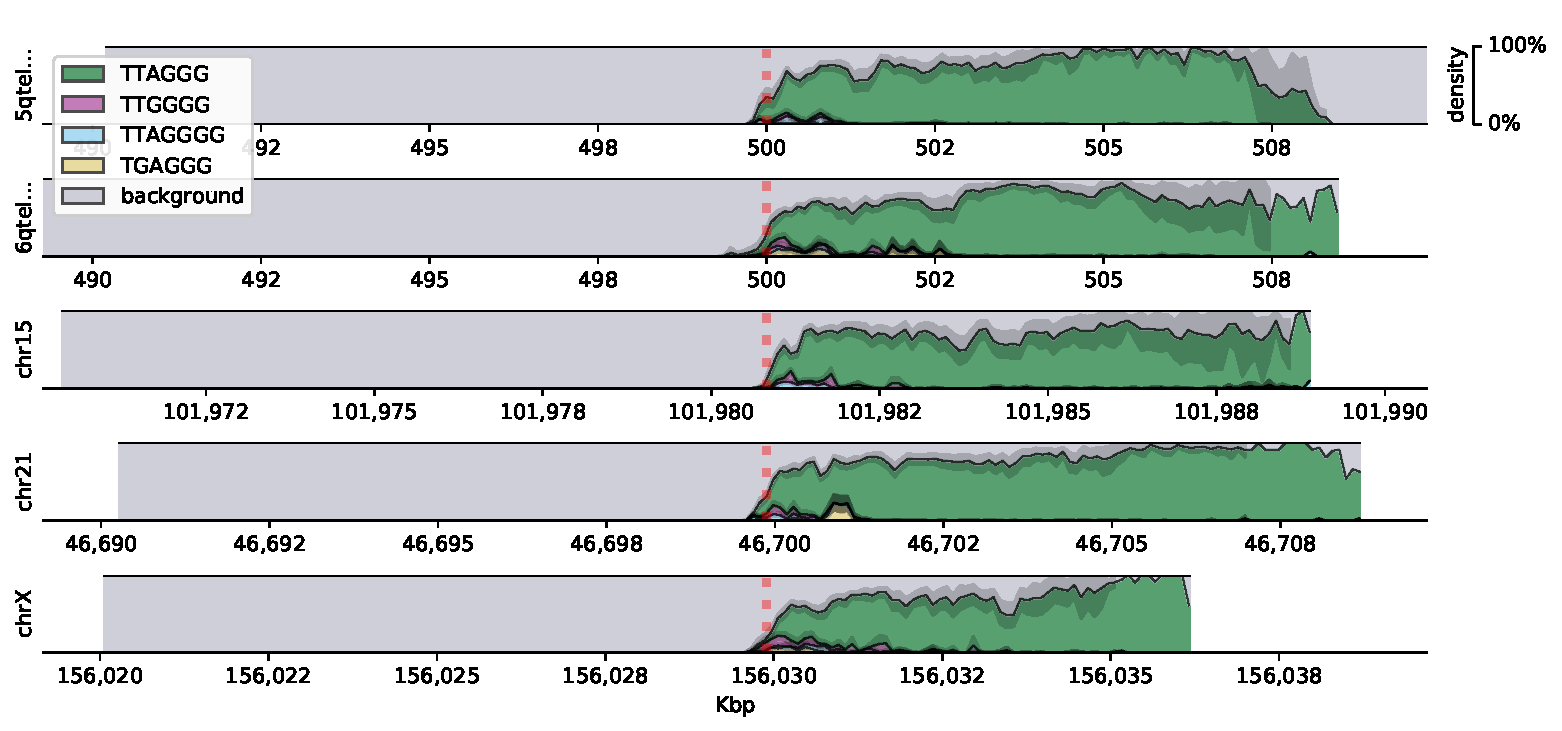
\includegraphics[width=\textwidth,keepaspectratio]{renders/figures/Figure-S4.pdf}
\end{figure}

\end{document}
